% !TEX TS-program = pdflatex
% !TEX encoding = UTF-8 Unicode

% This is a simple template for a LaTeX document using the "article" class.
% See "book", "report", "letter" for other types of document.

\documentclass{article} 
\usepackage[14pt]{extsizes} %задаем размер шрифта

\usepackage[utf8]{inputenc} % set input encoding (not needed with XeLaTeX)
\usepackage[T2A]{fontenc}
\usepackage[pages=some]{background}
\usepackage{graphicx} % support the \includegraphics command and options
\usepackage[most]{tcolorbox} % для управления цветом

\definecolor{sw}{RGB}{229,177,58} %Цвет текста звездных войн эпизода 1
\definecolor{sky_black}{RGB}{17,16,10} %Цвет ночного неба
% Настройка для рамки вокруг текста
\definecolor{block-gray}{gray}{0.90} % уровень прозрачности (1 - максимум)
\newtcolorbox{myquote}{colframe=sw, colback=black,grow to right by=-10mm,grow to left by=-10mm,
boxrule=2pt,boxsep=0pt} % настройки области с изменённым фоном

\usepackage{hyperref} %для гиперсылок
\usepackage{xcolor}

\backgroundsetup{
scale=1,
color=black,
opacity=1,
angle=0,
contents={%
  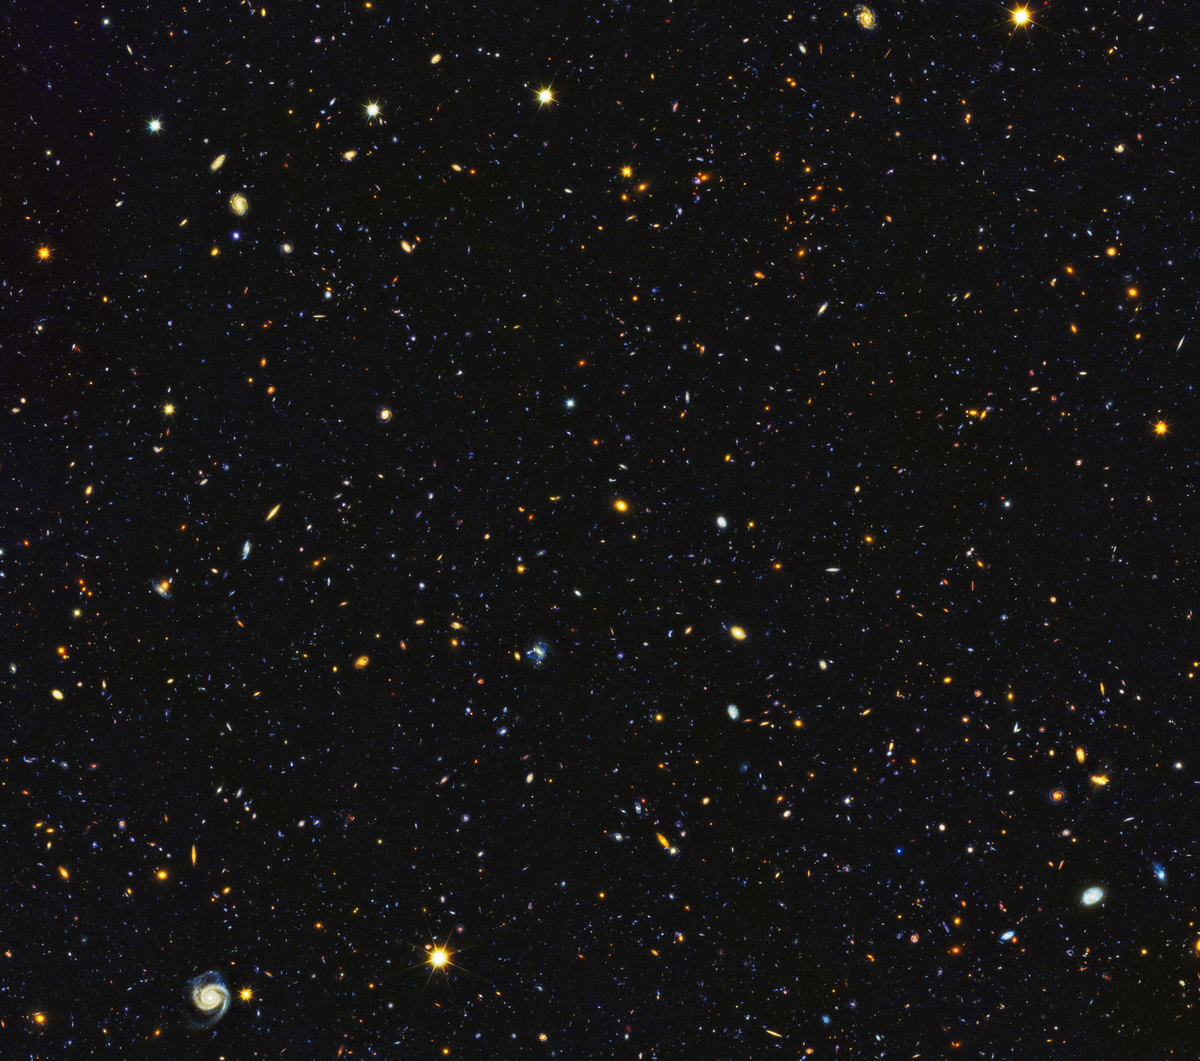
\includegraphics[width=\paperwidth,height=\paperheight]{imgs/stars_img.jpg}
  }%
}

\title{Забытый артефакт}
\author{SW Duncan's community}
%\date{} % Activate to display a give date or no date (if empty),
         % otherwise the current date is printed 

\color{sw}
\begin{document}
\pagecolor{sky_black}
\BgThispage
\maketitle %титульная страница
\newpage
\tableofcontents %оглавление
\newpage
\section{В поисках храма}

Описание посадки на планету.
\begin{myquote}
\color{sw}
\input{envs/planet.tex}
\end{myquote}
Персонажи могут искать храм:
1) С помощью жителей деревни, тогда перелестни на главу "С дипломатической миссией к каннибалам"
2) По воздуху, тогда перелестни на главу "Воздушный вояж"
3) Спуститься на землю и идти пешком до храма(тогда передистни на главу )
\subsection{Воздушный вояж}
В стандартной ситуации во время поиска храма на персонажей налетит буря, которая разобьет корабль.
В момент бури попроси пилота три раза бросить д20. Эти броски определят расстояние, на котором они сядут от храма.
Каждый бросок 7 и ниже(при этом не забудьте изменить число в соответствии с модификатором Ловкость) отдаляет игроков на 1 км от храма. При путешествии по джунглям от корабля до храма на каждом километре пути им встретится местная живность(подробнее смотри в главе про путешествие пещком <>). Если персонажи бросят все три кубика выше 7, то они сядут у подножия храма и могут сразу в него войти(далее смотри главу "Храм лорда ситхов").

\begin{myquote}
\color{sw}
\input{envs/fly_bad.tex}
\end{myquote}
\subsection{С дипломатической миссией к каннибалам}
Описание посадки на планету
\begin{myquote}
\color{sw}
\input{envs/landing.tex}
\end{myquote}

Описание деревни
\begin{myquote}
\color{sw}
\input{envs/village_far.tex}
\end{myquote}
В деревни главным действующим лицом является староста. Все жители деревни на любой вопрос будут отправлять персонажей к старосте. При первом подходе персонажей к деревне все жители деревни и староста выходят на границу деревнии. Здесь персонажи могут начать диалог.

В религии муйу практикуются жертвопринашения, однако можно приносить в жертву разумного только раз в 2 месяца, а последнее жертвопринашение было позавчера, но также можно делать это чаще, если разумные нарушат кодекс.
Персонажей принесут в жертву, если:
1) Они проявят неуважения к жителям деревни или старосте(к примеру оскорбят)
2) Услышат задание от старосты, согласятся его выполнить, но не выполнят
3) Войдут на территорию деревни без разрешения
4) Коснуться или наврядят алтарю в центре деревни
Никто из жителей не говорит персонажам эти условия. Игроки должны использовать интуицию, а мастер косвенно подсказывать.

Для предоставления проводника до храма староста потребует выполнить два задания:
1) Убить монстров в джунглях(обычное сражение)
2) Пройти лабиринт молодого воина(смотреть лабирит в главе \ref{lab_img})


Описание перехода от деревни к храму
\begin{myquote}
\color{sw}
\input{envs/village_to_temple.tex}
\end{myquote}

\section{Путешествие пешком}


\section{Храм лорда ситхов}
Описание храма
\begin{myquote}
\color{sw}
\input{envs/temple.tex}
\end{myquote}

Описание одних из стражей по пути в комнату ситхов.
\begin{myquote}
\color{sw}
Бродя по храму, вы наткнулись на комнату, полную злобных духов, возвращенных к жизни могучим ситхским лордом.
Пол комнаты покрыт застарелой кровью - явный признак темных ритуалов. Вероятно, описание самих ритуалов можно найти тут же, все стены комнаты исписаны странными символами, которые вы видели ранее.
Ваши шаги гулко раздаются по всему помещению, поэтому скрыться вряд ли получится.
Впереди видна массивная запертая дверь, за которой явно скрывается главная гробница. К сожалению, призраки не настроены вас туда пропустить.

\end{myquote}
Призракам не нанести урон бластерами или световыми мечами.
Бороться с ними придется на ментальном фронте, объединив усилия и создавая Волны тьмы, отправляющие призраков назад в Бездну.
Кроме того, вам может помочь Светлый дух, вызвав Стену света (если, конечно, вам не противно применение Светлой стороны в своем присутствии)
Если подпустить призрака слишком близко к себе, он сможет овладеть вашим разумом и свести с ума, так что будьте осторожны и следите за своими товарищами - любой из них может вонзить меч вам в спину.

\section{Дополнительно}
\label{5000}
Изображение лабиринта молодого воина.
Вход слева сверху.
Выход снизу справа.
Всеми остальными обозначениями пренебречь.
Рисовать лабиринт вместе с перемещением игроков, при том только ту часть лабиринта, которую игроки могут видеть.
\newline
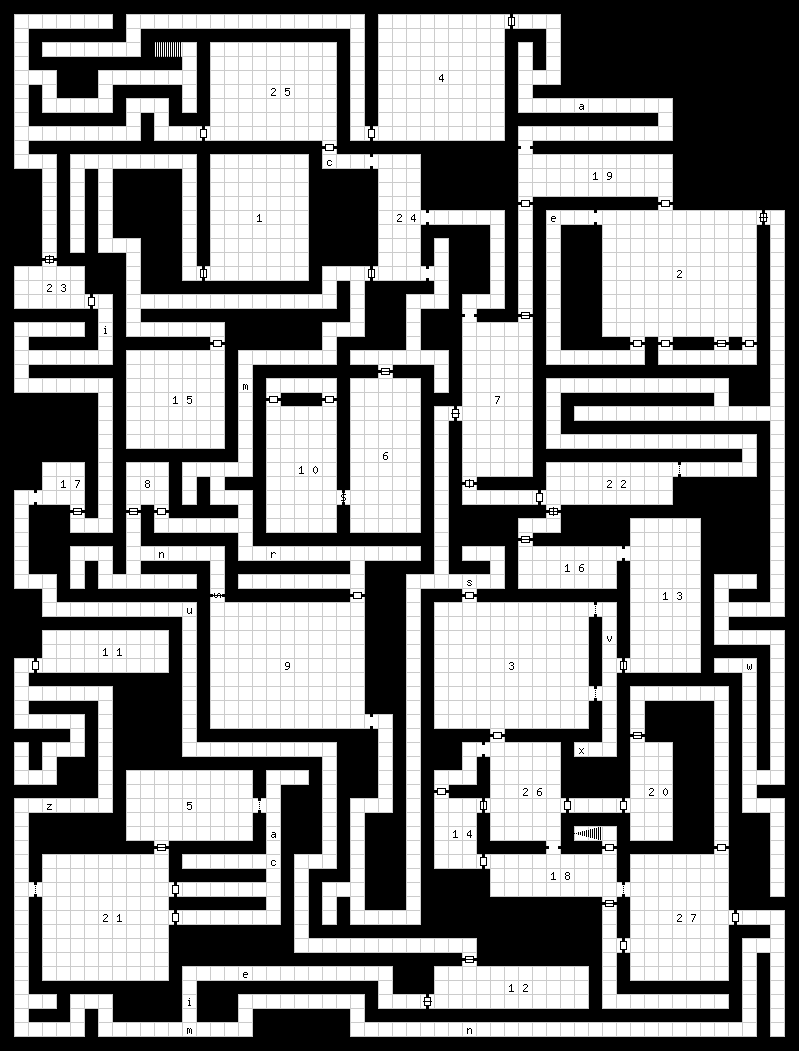
\includegraphics[width=1\textwidth]{imgs/labirint} \label{lab_img}
\end{document}
